\section{Evaluation Crowdsourcing-System}
\subsection{Kandidaten}
\begin{itemize}
	\item MapRoulette\footnote{\url{http://maproulette.org/}} 
	\item To-Fix\footnote{\url{http://osmlab.github.io/to-fix/\#/task/tigerdelta}}
\end{itemize}

\subsection{MapRoulette}
MapRoulette verwendet für ihre Challenges und Tasks ein einfaches JSON Format. Der erstellt werden Challenges mittels POST und mit PUT können diese upgedatet werden.

\subsection*{Beispiel Challenge}
\begin{tabbing}
    \hspace*{4cm}\=\hspace*{5cm}\= \kill
    Erstellen: \> POST /api/admin/challenge/<slug>  \\
    Updaten: \> PUT /api/admin/challenge/<slug> \\
    Challenge JSON: \\
\end{tabbing}		
\begin{python}
{
  "title": "Repair Motorways",
  "description": "Repair all motorways",
  "blurb": "The idea is to repair all motorways",
  "help": "Repair the ways where it is broken on the map",
  "instruction": "Look at the map for broken pieces.",
  "active": true,
  "difficulty": 2
}
\end{python}

\subsection*{Beispiel Task}
\begin{tabbing}
    \hspace*{4cm}\=\hspace*{5cm}\= \kill
    Erstellen: \> POST /api/admin/challenge/<slug>/task/<task\_identifier> \\
    Updaten: \> PUT /api/admin/challenge/<slug>/task/<task\_identifier> \\
    Challenge JSON: \\
\end{tabbing}
\begin{python}
{ 
  "instruction" : "This is a hard task!",
  "geometries" : {
    "type": "FeatureCollection",
    "features": [
      { "type": "Feature",
        "geometry": 
        { "type": "Point", 
          "coordinates":[-41.4710170873565,31.235521774136]
        },
        "properties": {"osmid": 12345}
      }
    ]
  }
}
\end{python}	

\subsection{To-Fix}
To-Fix verwendet für ihre Task ein CSV Format, welches direkt über das grafische Benutzerinterface publiziert werden kann.
\subsection*{Beispiel CSV}
\begin{python}
object_type,object_id,st_astext
way,51446110,POINT(-94.4176451 43.3273692)
way,187403368,POINT(32.9369086 2.1997495)
way,220866128,POINT(-68.5 49.647521)
way,223982938,POINT(18.4823301 59.6732909)
way,109819283,POINT(-83.1888421 40.0485764)
\end{python}


\subsection{Evaluationsmatrix}
Um die beiden Kandidaten zu vergleich haben wir eine Evaluationsmatrix erstellt, dabei haben wir diverse für uns relevante Kriterien erarbeiten und diesen jeweils auf einer Skala von 1 bis 10 gewichtet.
In einem zweiten Schritt haben wir den Kandidaten für die jeweiligen Kriterien Punkte vergeben.

\begin{figure}[ht]
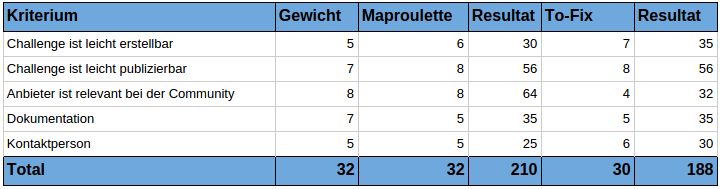
\includegraphics[width=\textwidth]{images/croud_evol_matrix.png}
\caption[Evaluationsmatrix]{Evaluationsmatrix}
\end{figure}

\subsubsection{Resultat}
Beide Kandidaten haben Vor- und Nachteile, wie aus der Evaluationsmatrix ersichtlich ist. Für uns ist das wichtigste Kriterium, wie relevant der Anbieter bei der Community ist, was sich dann auch im Resultat stark ausgewirkt hat. Da MapRoulette Challenges gerne abgearbeitet werden, tendieren wir für diesen Kandidaten.  